\chapter{Avaliação} \label{ch:evaluation}

Este Capítulo apresenta resultados comparativos da solução desenvolvida com a 
aplicação original. A Seção \ref{sect:methodology} apresenta detalhes da 
metodologia de avaliação, a Seção \ref{sect:results} disserta sobre os 
resultados e a Seção \ref{sect:failures} fala sobre casos de falha encontrados 
durante os testes.


\section{Metodologia de Avaliação} \label{sect:methodology}

Os experimentos foram realizados no Parque Computacional de Alto Desempenho 
(PCAD) da UFRGS. Eles ocorreram nos nós de computação \mytexttt{draco}, cuja 
configuração de um nó é mostrada na Tabela \ref{tab:draco_config}. Todos os nós 
do cluster possuem a mesma configuração, com exceção de um que não foi utilizado.

\begin{table}[H]
\centering
\small
%\footnotesize
\begin{tabular}{l c} \toprule
\textbf{Parâmetro}  &  \textbf{Configuração} \\ 
\midrule
Processador     & 2 x Intel Xeon E5-2630 (Q1'12) Sandy Bridge, 2,5 GHz  
\\
Número de Núcleos Físicos    & 16  \\
Número de Núcleos Lógicos   & 32   \\
Memória       & 64 GB DDR3 RAM   \\
Rede	      & Ethernet 10 Gigabit \\
\end{tabular}
\caption{Configurações de um nó \mytexttt{draco}.}
\label{tab:draco_config}
\end{table}


A Figura \ref{fig:experiment_arch} exibe a arquitetura que foi seguida durante 
os experimentos. Como o Spark acessa dados direto do HDFS, primeiramente 
executamos o Hadoop. Um dos nós era responsável por executar o \textit{namenode} 
e também executava uma instância de \textit{datanode}. Os demais executavam 
apenas \textit{datanodes}.


\begin{figure}[ht]
\centerline{
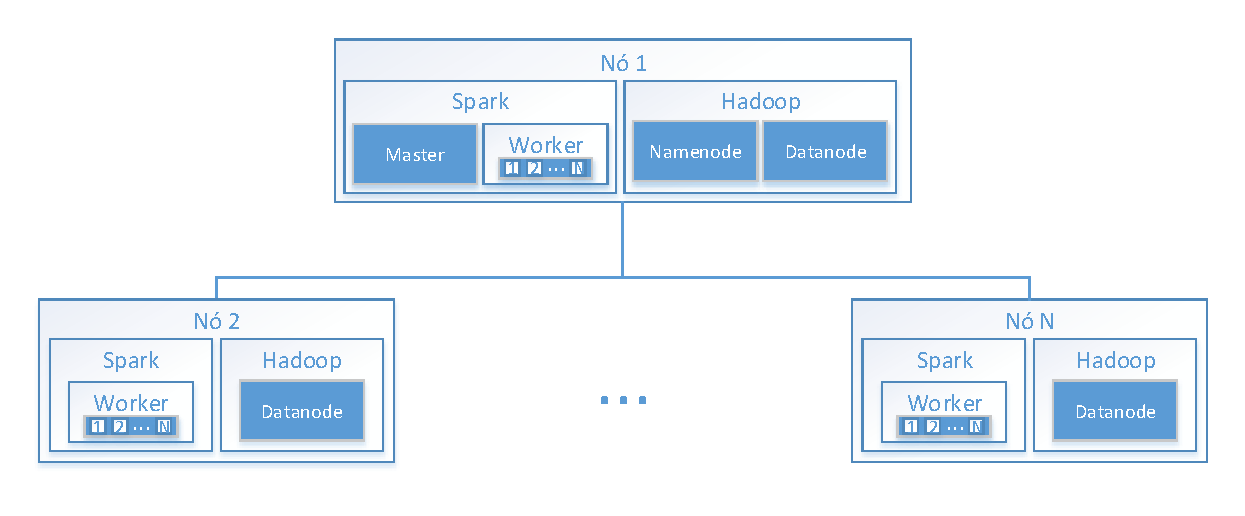
\includegraphics[width=0.9\textwidth]{./img/experiments_arch.pdf}}
 \caption{Arquitetura de aplicações durante os experimentos.}
 \label{fig:experiment_arch}
\end{figure}


O gerenciador de cluster utilizado foi o do próprio Spark ao invés do YARN. 
Essa decisão foi tomada durante os testes pois seus arquivos de registro 
mostraram informações mais claras sobre o que estava ocorrendo. A abordagem 
utilizada para ele foi similar àquela utilizada no Hadoop, um nó executou 
como mestre e trabalhador enquanto os demais executaram apenas como 
trabalhadores. 

Cada trabalhador do Spark instancia N executores, responsáveis 
por processar tarefas. Cada um destes possui uma quantidade de núcleos e uma 
quantidade de memória dedicada. Durante os experimentos, parametrizamos a 
\textit{engine} para que cada trabalhador utilizasse 15 executores, cada um com 
2 núcleos e 4 GB de memória para processamento de tarefas.

Realizamos testes com 1 nó, utilizando a aplicação original, 15 executores em 1 
nó, 30 executores em 2 e 45 executores em 3 nós, utilizando a aplicação 
modificada. Cada teste foi configurado para executar 30 vezes para garantir a 
confiabilidade de seus resultados, todavia, houveram casos isolados de problemas 
de execução que não afetaram as tendências gerais observadas.


\section{Experimentos e Resultados} \label{sect:results}

A carga de trabalho dos experimentos já no formato CSV, entrada para a fase de 
pré-processamento no StarVZ, tinha um somatório de 12 GB. Ela consiste em 
rastros de execução de uma aplicação cholesky e foi escolhida pois era a maior
entrada que tínhamos no momento. O tamanho de cada um dos arquivos pode ser 
visualizado na Tabela \ref{tab:input_sz}.

\begin{table}[H]
\centering
\small
\begin{tabular}{l c} \toprule
\textbf{Arquivo}  &  \textbf{Tamanho} \\ 
\midrule
state.csv	& 6.8 GB \\
variables.csv  	& 2.5 GB \\
link.csv       	& 304 MB \\
dag.csv        	& 270 MB \\
entities.csv	& 73 KB \\
events.csv	& 1.8 GB \\
\textbf{Total}  & 12 GB  \\
\end{tabular}
\caption{Detalhamento da carga de trabalho.}
\label{tab:input_sz}
\end{table}

Durante a implementação, optou-se por manter o processamento de entities
no formato sequencial pois esse arquivo armazena apenas informações de 
plataforma e por isso, costuma não passar da ordem de tamanho de KB. Podemos 
observar que isso se confirma nesta carga de trabalho.

Foram executadas 30 repetições em cada teste, todavia, os experimentos com o 
Spark apresentaram problemas em algumas execuções, discutidos na Seção 
\ref{sect:failures}. Tivemos três testes com problemas ao executar com 15 
executores enquanto com 30 e 45, tivemos apenas um. Nesses casos, consideramos 
apenas aquelas que processaram com sucesso (27, 29 e 29 repetições, 
respectivamente). 

A Figura \ref{fig:total_full} mostra a média do tempo total de execução dos 
experimentos e o erro padrão no topo da barra (intervalo de confiança 
de 99,7\%) em função do paralelismo em cada nó. A execução original 
de forma sequencial, levou em média 1489,02 segundos para completar o 
processamento. Já as execuções com a aplicação adaptada para utilizar o Spark, 
com 15 executores em 1 nó levou em média 708,17 segundos, com 30 em 2 nós, 
460,81 segundos e 45 em 3, 385,44 segundos. Isso consiste em um \textit{speedup} 
de respectivamente 2,10x, 3,23x e 3,86x em relação ao original.

\begin{figure}[ht]
\centerline{
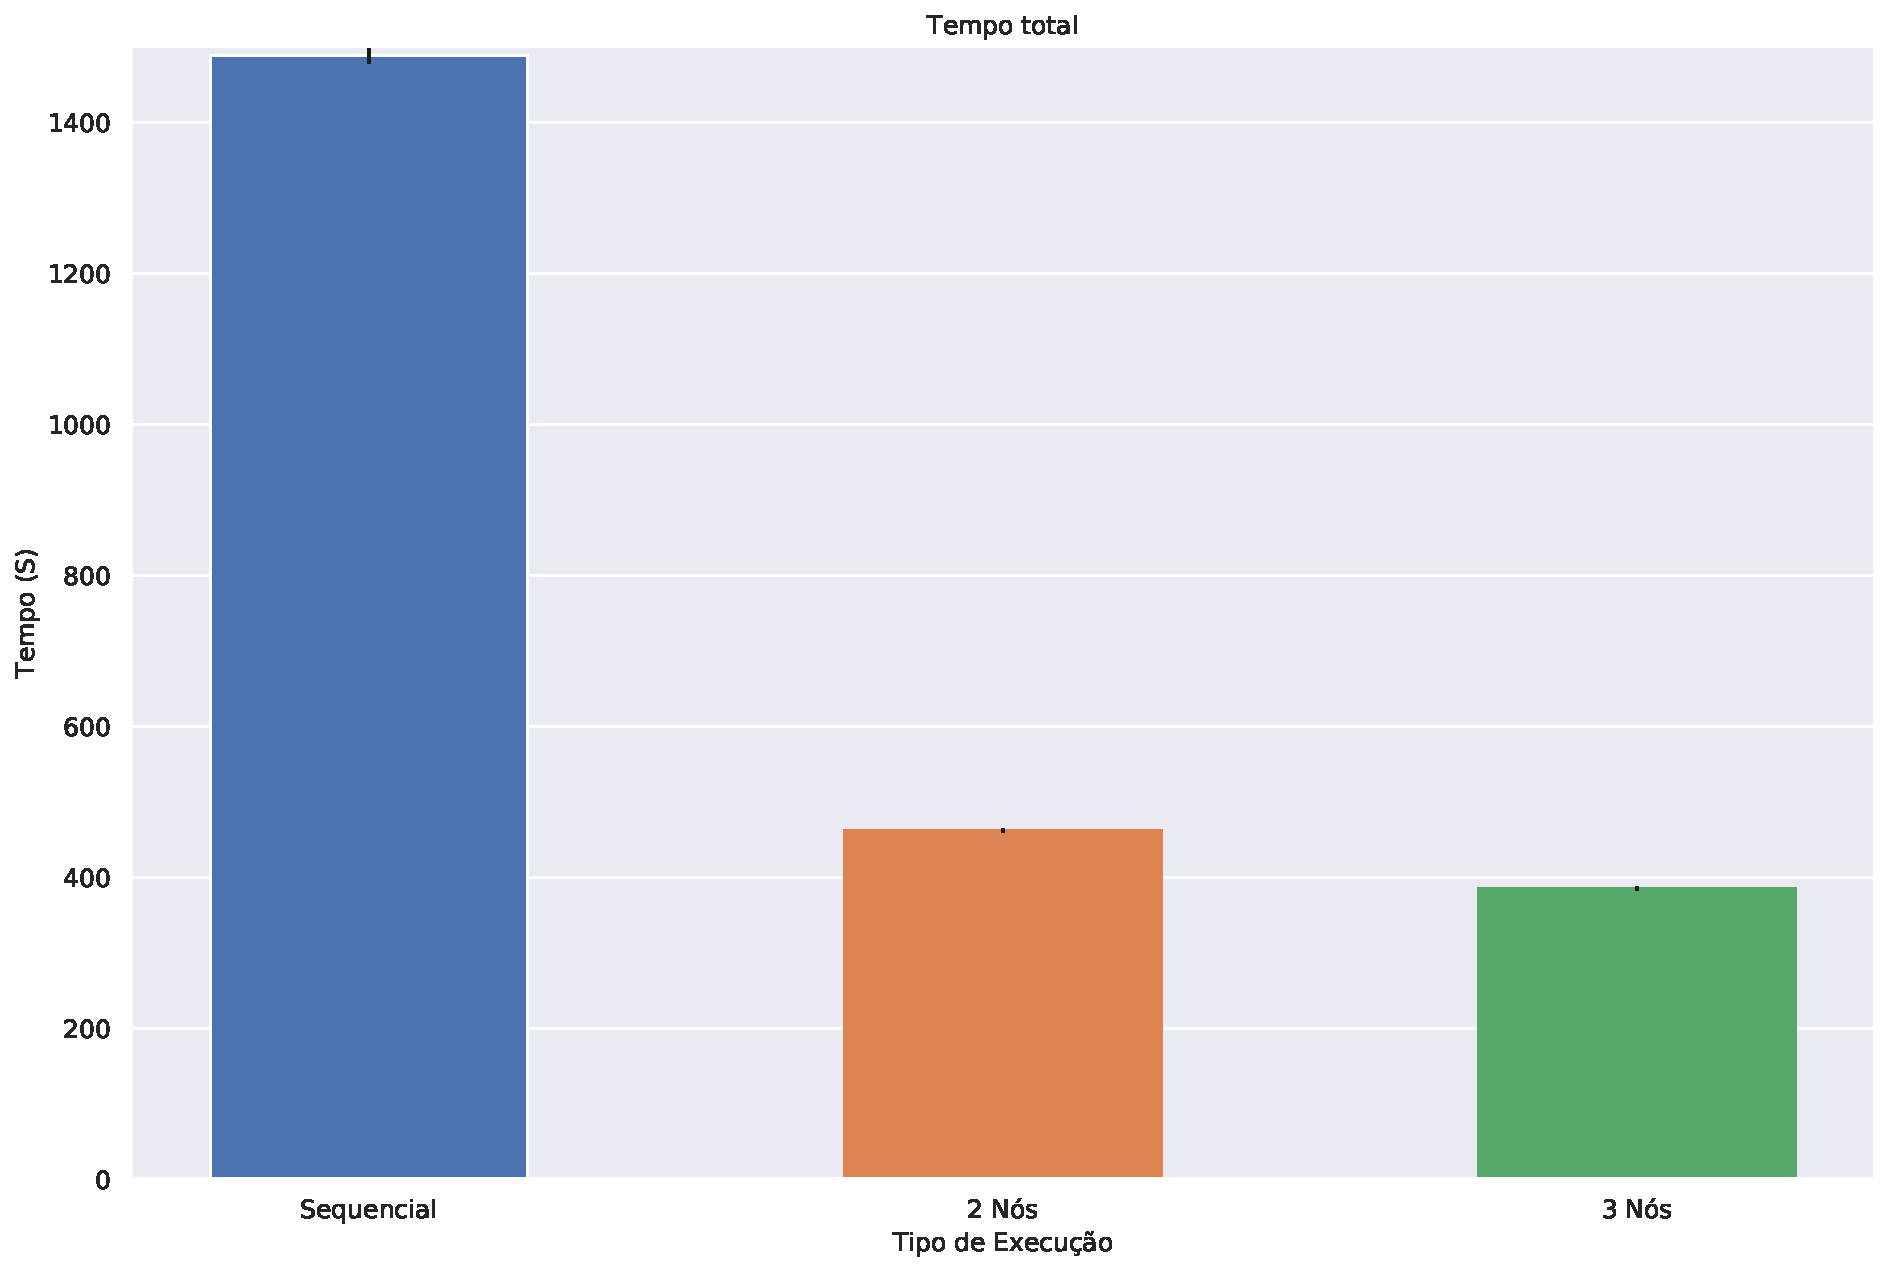
\includegraphics[width=0.8\textwidth]{./img/total.pdf}}
 \caption{Tempo total de execução da aplicação.}
 \label{fig:total_full}
\end{figure}


Segmentamos a análise pelas etapas exibidas na Figura 
\ref{fig:spark-starvz-flow}, seus tempos de execução podem ser visualizados na 
Figura \ref{fig:total_step} e consultados com mais detalhes na Tabela 
\ref{tab:total_step}. Analisando os resultados e o código, conseguimos 
separar as etapas em quatro grupos.

O primeiro e mais trivial deles, é o grupo em que não houve praticamente 
nenhuma alteração de código e tempo de execução. É o caso do tratamento de 
entities, que foi apenas convertido para uma tabela Spark para posterior 
gravação no HDFS.

\begin{figure}[H]
\centerline{
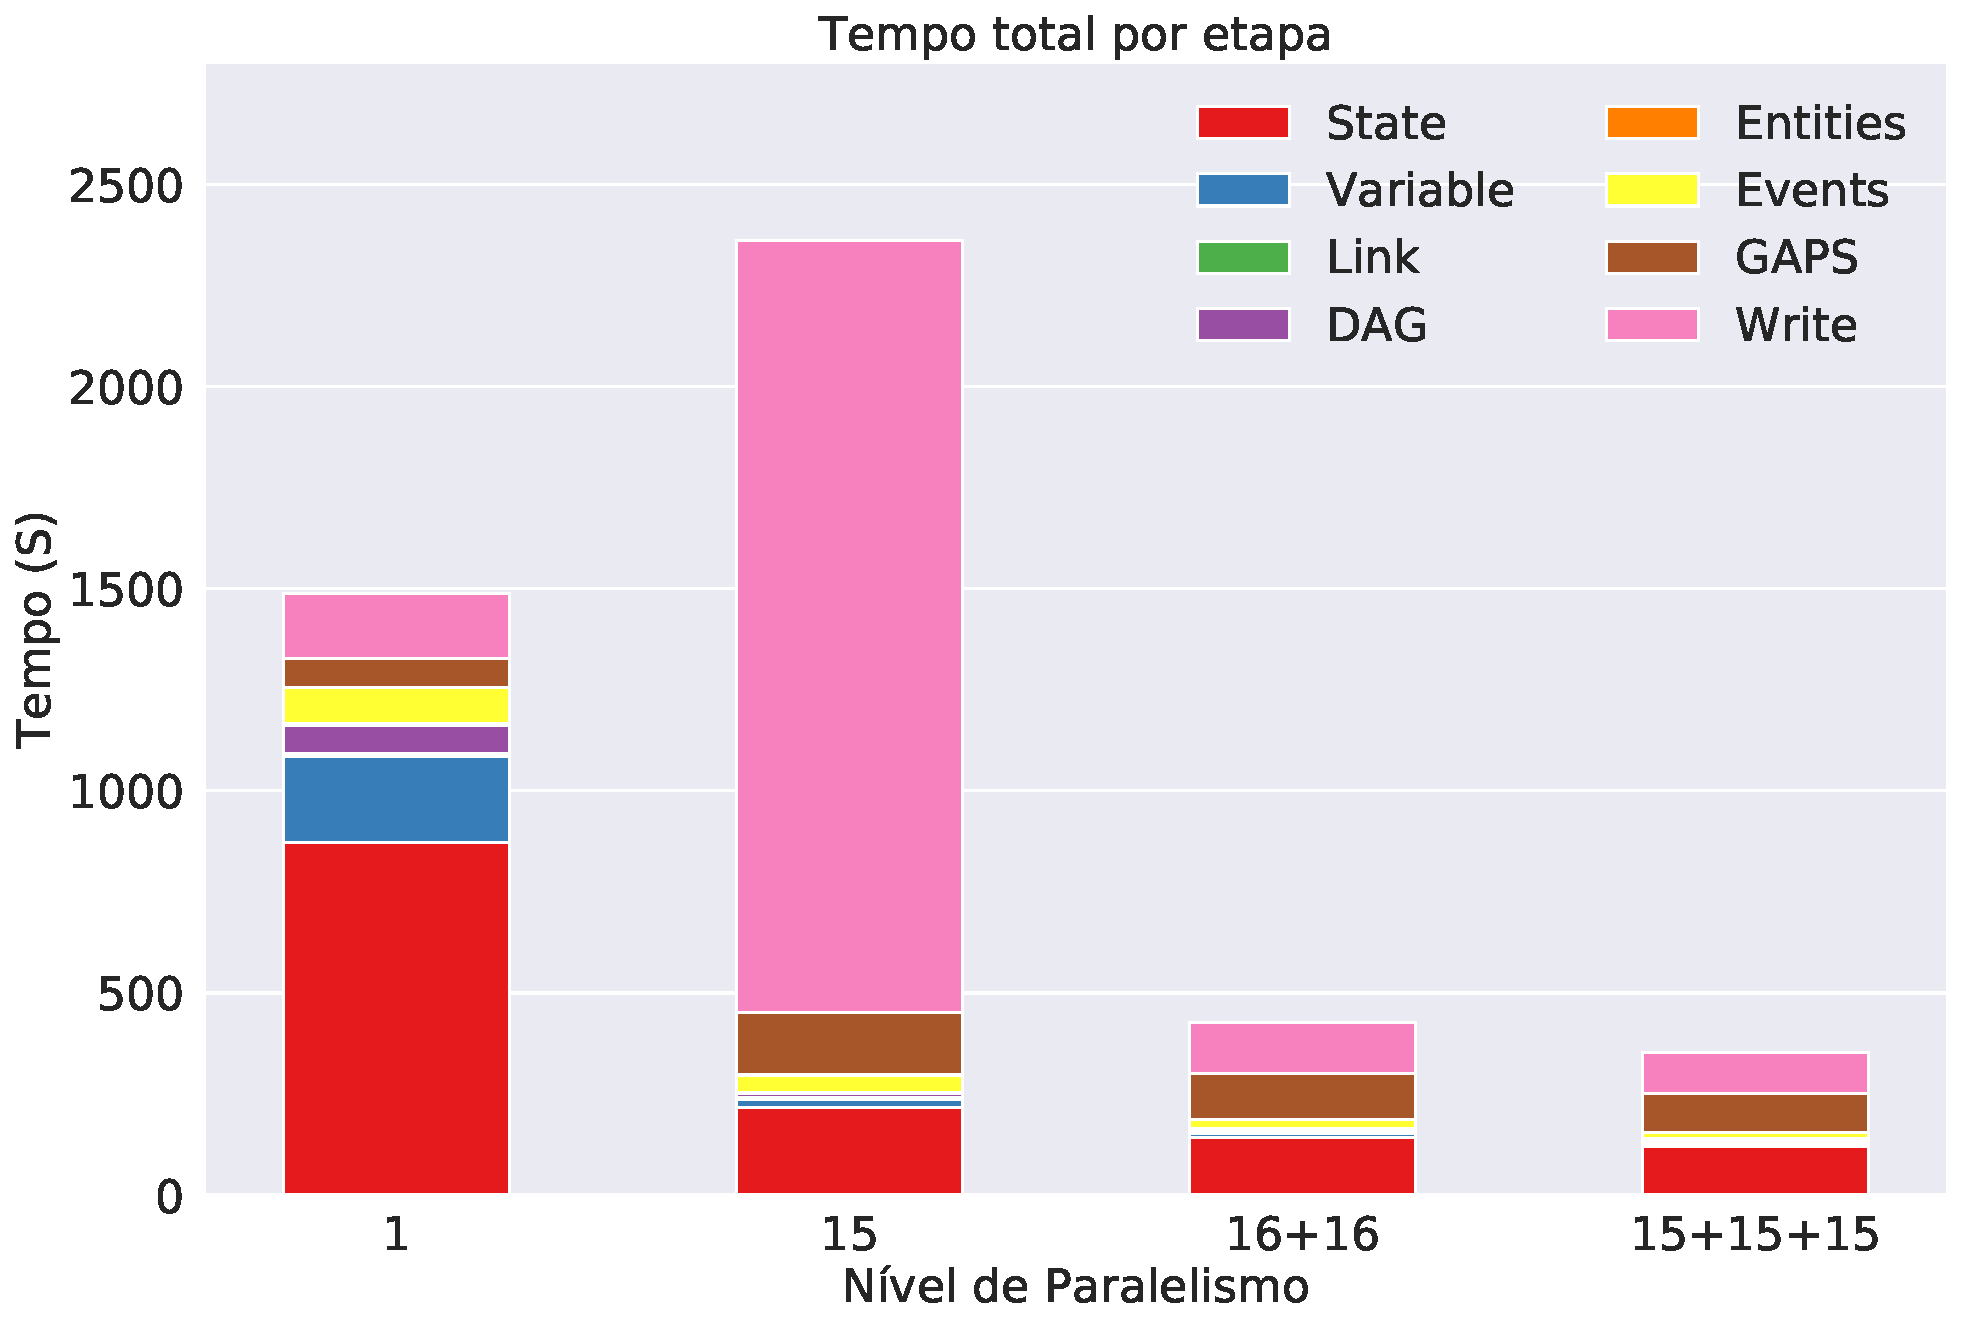
\includegraphics[width=0.8\textwidth]{./img/total_step.pdf}}
 \caption{Tempos de execução segmentados por etapas.}
 \label{fig:total_step}
\end{figure}


\begin{table}[ht]
\centering
\small
\begin{tabular}{l c c c c} \toprule
\textbf{Etapa}  & \textbf{1} & \textbf{15} & \textbf{15+15} & 
\textbf{15+15+15}\\ 
\midrule
State		& 873.31 & 215.93 & 142.15 & 119.20\\
Variable  	& 210.77 & 21.17  & 10.44  & 7.50 \\
Link      	& 8.93   & 4.59   & 3.84   & 3.53 \\
DAG        	& 69.14  & 10.10  & 7.58   & 6.76 \\
Entities	& 3.07   & 2.42   & 2.31   & 2.30 \\
Events		& 89.87  & 42.68  & 22.65  & 15.91\\
GAPS		& 71.51  & 154.03 & 110.83 & 95.22\\
Write		& 162.19 & 211.06 & 125.40 & 102.87\\
\end{tabular}
\caption{Tempos médios de execução, em segundos.}
\label{tab:total_step}
\end{table}

O segundo grupo identificado, foram manipulações que executaram apenas 
transformações (operações \textit{Lazy}) no Spark \cite{ref:sparkbook} durante 
seu processamento. Estas constroem um plano de operações a serem aplicadas nos 
dados, todavia, a \textit{engine} só irá executá-lo quando estritamente 
necessário (quando uma ação for realizada). Neste grupo enquadram-se as tabelas 
que observou-se um \textit{speedup} muito grande, como é o caso de variable que 
apresentou 9,95x, 20,18x, 28,10x comparando-se as execuções com Spark com a 
execução Sequencial. A etapa que lida com o DAG também teve ganhos 
consideráveis, apresentando \textit{speedups} de 6,84x, 9,12x e 10,22x. Os 
ganhos de link foram menos significativos, pois seu tempo original já é 
pequeno, concluímos que ele pertence a este grupo pela análise do código de seu 
tratamento.

O terceiro grupo identificado foram transformações que de alguma forma ativaram 
uma ação no Spark durante seu processamento. Tais operações fazem com que a 
\textit{engine} efetivamente manipule os dados \cite{ref:sparkbook} não sendo 
do tipo \textit{Lazy} como as transformações. Esse grupo consiste nos 
tratamentos de state e events, nos quais tivemos um ganho inferior ao segundo 
grupo. Os ganhos observados para events foram de 2,10x, 3,96x e 5,64x, enquanto 
que para state tivemos 4,04x, 6,14x e 7,32x.

O último grupo, corresponde apenas ao Cálculo de GAPS. Essa operação foi 
levantada durante a implementação como um ponto de atenção, devido ao seu tempo 
ter aumentado de forma considerável em experimentos locais. Olhando para os 
tempos de execução temos, em segundos, 71,51 na execução sequencial, 154,03 na 
com 15 executores utilizando Spark, 110,83 com 30 executores e 95,22 utilizando 
45 executores. Acreditamos que isso seja decorrente das ações Spark realizadas 
em tabelas geradas por junções de forma recursiva, utilizadas nesta etapa. Para 
identificar o ponto exato que causa essa perda de desempenho, são necessários 
mais testes.

Por fim, temos a escrita dos dados no sistema de arquivos distribuído. Nessa 
etapa pode-se observar que o ganho não é tão grande pois é nela que todos os 
planos de transformações montados nas etapas anteriores serão efetivamente 
executados sobre os dados. Isso é decorrente da escrita de uma tabela ser
considerada uma ação e portanto, exige que transformações sejam realizadas.
Pode-se observar, tanto na Tabela 
\ref{tab:total_step} quanto na Figura \ref{fig:total_step} que o tempo de 
execução com o Spark utilizando 15 executores é pior do que a execução 
sequencial. Depois dela, temos pequenos \textit{speedups} de 1,29x e 1,57x.

Portanto, podemos concluir que a portagem do arcabouço StarVZ para executar 
sobre o Spark gerou ganhos consideráveis. Há outras diversas avaliações para 
serem realizadas, algumas serão enumeradas no próximo Capítulo.


\section{Casos de Falha} \label{sect:failures}

Ocorreram algumas falhas de execução durante os testes comparativos entre a 
versão sequencial e distribuída. Nos logs da aplicação (no \mytexttt{Processo 
Driver} do Spark), é reportado que não foi possível criar uma conexão Spark. Nos 
logs do nó mestre não há registros de que houve a recepção de uma requisição 
para criar a aplicação, o que indica que a conexão efetivamente não foi criada. 
Devido ao comportamento observado, acreditamos que seja algum recurso que não 
foi liberado entre execuções, pois o tempo entre finalizar uma execução e 
iniciar outra é de apenas milissegundos. Para determinar a causa exata do 
problema, é necessário uma investigação mais aprofundada que deixamos 
como trabalhos futuros.

Foi disponibilizado uma carga de trabalho de 116 GB. Ao tentar executar a versão 
sequencial houve um erro de alocação de memória, o que era esperado tendo em 
vista que as máquinas possuem apenas 64 GB de memória. Todavia, executando a 
versão com Spark, ele também não completou a aplicação. Durante o processamento 
de State, o processo é bloqueado e encerrado por \textit{timeout} 
(expiração de tempo de limite). Não houve tempo durante o trabalho para 
corrigir os problemas observados e rodar a aplicação com essa carga de 
trabalho, deixando isso também como um item para trabalhos futuros.
